\section{Results}
\label{sec:results}
Because the men would hang around the corner on windy days \cite{dresses}, a windy day was simulated with a wind speed of 9 $ms^-1$. To get a relatively accurate simulation, a iteration convergence of $1\cdot10^-4$ was recommended to us. \\\
\indent %
In order to adequately judge the wind around the building, an overview is created by plotting the streamlines at 3 different heights. These are shown at the bottom(figure \ref{fig:streamlinesbottom}), around the middle(figure \ref{fig:streamlinesmid}) and at the top(figure \ref{fig:streamlinestop}) of the Flatiron building and can be found in appendix \ref{sec:streamlines} \\
To check if women's ankles would really show, a plot of the velocity in the z-direction, the pressure and the turbulent kinetic energy were made at a height of 1.37 meter (this was the lowest the program could go). These a shown in figures x y z. \\
\begin{figure}[h!]
\centering
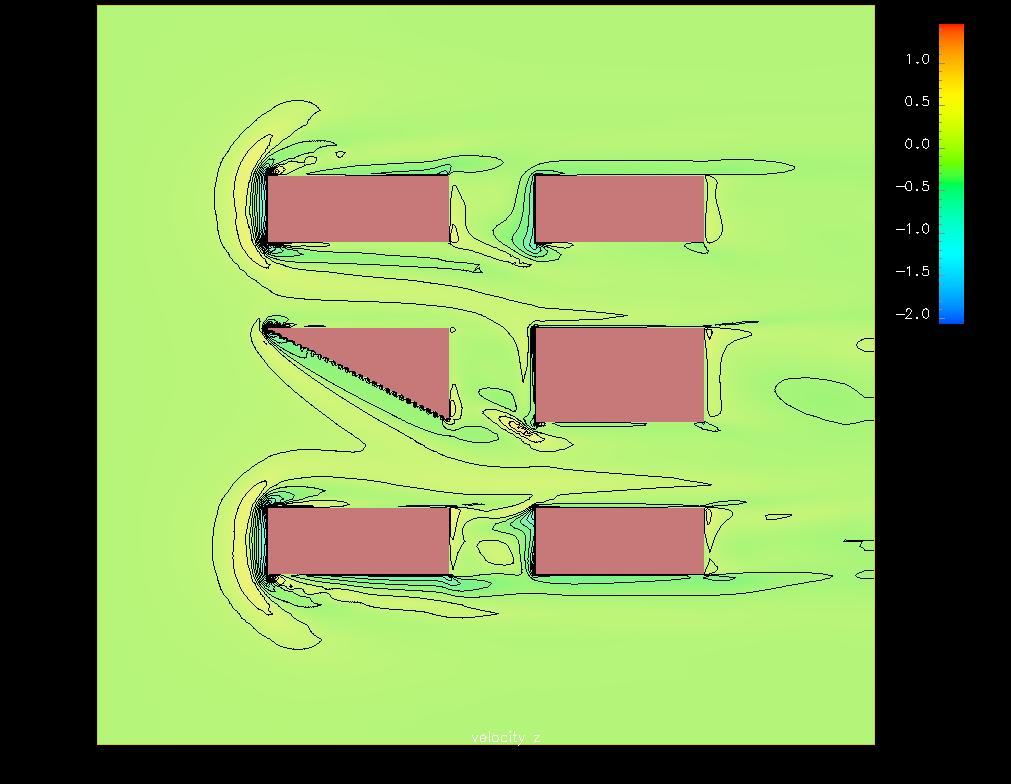
\includegraphics[width = \textwidth]{zvelocity.png}
\caption{Velocity in the z-direction around the Flatiron building at z=1.37 m}
\label{fig:zvelocity}
\end{figure}\\
\begin{figure}[h!]
\centering
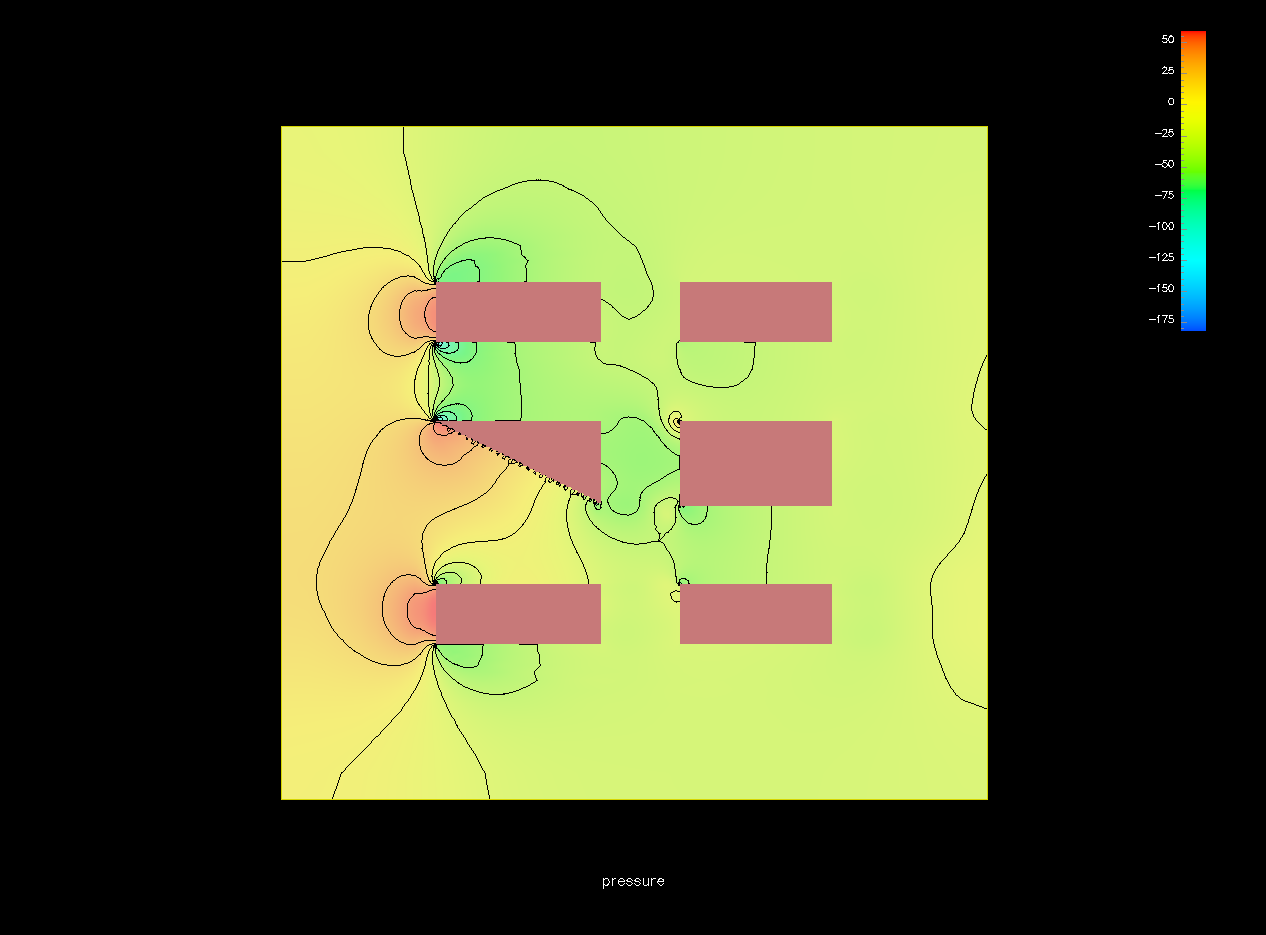
\includegraphics[width = \textwidth]{zpressure.png}
\caption{Pressure distribution(in Pa) around the Flatiron building at z=1.37 m}
\label{fig:zpressure}
\end{figure}\\
\begin{figure}[h!]
\centering
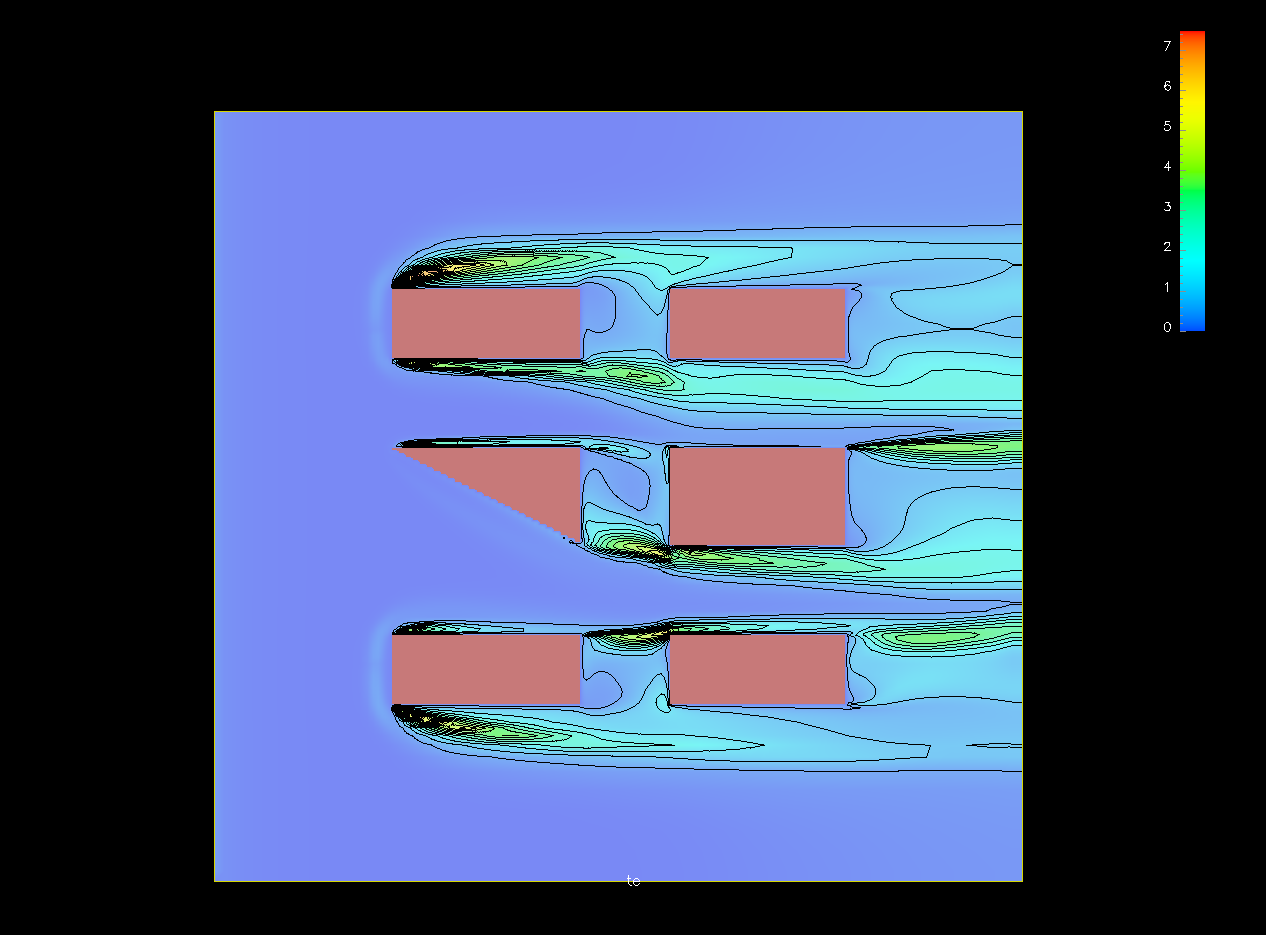
\includegraphics[width = \textwidth]{zenergy.png}
\caption{Turbulent kinetic energy(in $m^2s^{-2}$) around the Flatiron building at z=1.37 m}
\label{fig:zenergy}
\end{figure}\\